\section{Apariția noțiunii de algoritm genetic} 
 
Algorimii genetici\footnote{Adaptare după \textit{Genetic Algorithms: An Overview}, Melanie Mitchell, 1995.} au fost introduși de către John Holland în 1960 și dezvoltați, ulterior, alături de colegii de la Universitatea din Michigan, între anii 1960 și 1970. Holland urmărea înțelegerea fenomenului de adaptare întâlnit în natură și implementarea unor mecanisme adaptive care să fie utilizate în practică, în contextul programării. Cartea publicată de acesta în 1975, \textit{Adaptation în Natural and Artificial Systems} (Holland, 1975/1992) prezintă algoritmii genetici drept abstractizări ale evoluției biologice și oferă un cadru teoretic pentru dezvoltarea acestora.

Algoritmii genetici ai lui Holland sunt metode de a trece de la o populație de cromozomi (e.g., șiruri de biți care reprezintă soluții candidat pentu o problemă) la o nouă populație, prin folosirea selecției, alături de operatorii inspirați din genetică: încrucișare, mutație, inversiune. Cea din urmă este rar folosită în practică.

TODO: DE AFLAT CUM SE IMPLEMENTEAZA, TOTUSI, INVERSIUNEA \\

\begin{quote} 
	\textit{Computer programs that "evolve" in ways that resemble natural selection can solve complex problems even their creators do not fully understand.}
	\begin{flushright}
		John H. Holland 
	\end{flushright}
\end{quote}

\clearpage

Algoritmii genetici au fost creați în încercarea de a imita procese specifice evoluției naturale, cum ar fi lupta pentru supraviețuire și moștenirea materialului genetic. Putem privi evoluția drept strategia abordată de speciile biologice pentru a căuta soluții cât mai potrivite, adaptate condițiilor schimbătoare, într-un număr foarte mare de posibilități. Această abordare poate fi utilizată în rezolvarea problemelor de optimizare, atunci când metodele clasice exhaustive nu se dovedesc eficiente. 
 
Noțiunea de algoritm genetic nu este definită în mod riguros\cite{introduction_by_melanie_mitchell}, însă toate metodele ce poartă această denumire au în comun următoarele: populația este formată din cromozomi, selecţia este făcută pe baza rezultatelor funcției de optimizat, încrucișarea a doi \textit{cromozomi părinți} produce doi \textit{cromozomi copii}, mutația se aplică \textit{cromozomilor copii}. 

\section{Terminologie}

\begin{itemize}
	
	 \item Soluțiile candidat sunt adesea codificate în forma unor șiruri de biți și se mai numesc \textbf{cromozomi} sau \textbf{indivizi} ai populației. Fiecare bit este echivalentul unei gene. 
	 
	 \item Genele sunt informațiile stocate de către cromozomi. 
	 
	 \item \textbf{Populația}, care va fi urmărită în procesul său evolutiv, este alcătuită din mai mulți cromozomi. 
	 
	 \item Fiecare \textbf{generație} marchează câte o etapă din evoluția populației inițiale. 
	 
	 \item Pentru a trece de la o generație la alta, apelăm la noțiunea de \textbf{reproducere}. În alcătuirea următoarei generații, se pornește de la populația actuală, pe care o supunem unui proces de \textbf{selecție}. Pentru a face analogia cu fenomenul de supraviețuire a celor mai adaptați indivizi, măsurăm cromozomii cu ajutorul unei \textbf{funcții de optimizat}. O valoare ridicată a acestei funcții este interpretată ca o bună adaptare la mediu a individului.  
	 
	 \item Pentru explorarea spațiului de soluții, indivizii selectați suferă modificări. Sunt supuși \textbf{încrucișărilor} și \textbf{mutațiilor}. 
	 
	 \item Încrucișarea combină genele a doi \textit{cromozomi părinți}, rezultând doi \textbf{moștenitori}. Există mai multe variante: cu un punct de tăiere, ales aleator (în care un moștenitor este alcătuit dintr-o porțiune de cromozom de la primul părinte și o porțiune de la al doilea), cu mai multe puncte de tăiere și uniformă (unde fiecare genă este selectată probabilist de la unul din cei 2 \textit{cromozomi părinți}). 
	 
	 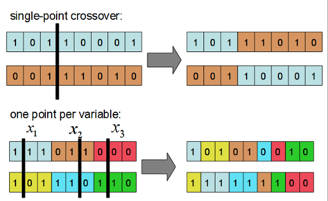
\includegraphics[
		 width=10cm,
		 height=6cm,
		 keepaspectratio
	 ]
	 {imagini/incrucisare.png}\\
	 
	 \item Mutația alterează gene alese arbitrar dintr-un cromozom. Numărul de gene afectate poate varia. 
	 
	 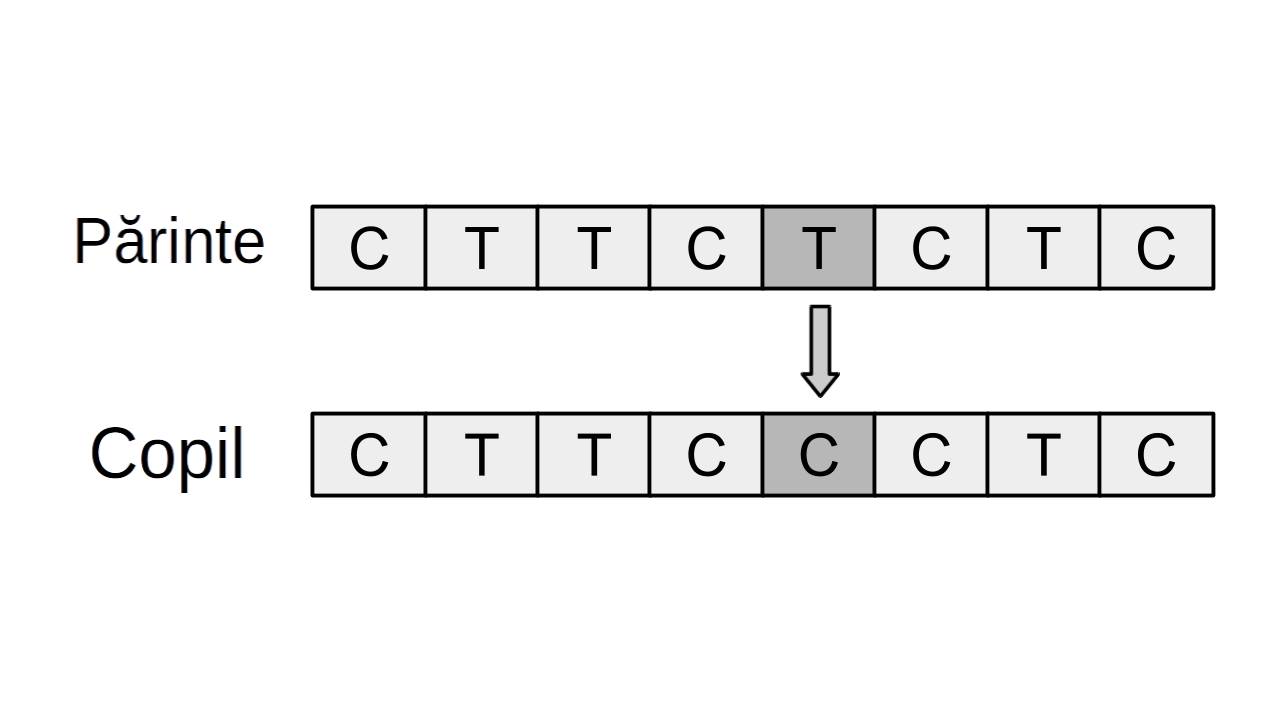
\includegraphics[
		 width=10cm,
		 height=6cm,
		 keepaspectratio
	 ]
	 {imagini/mutatie.png}\\
	
\end{itemize}

\section{Schema generala a unui algoritm genetic}

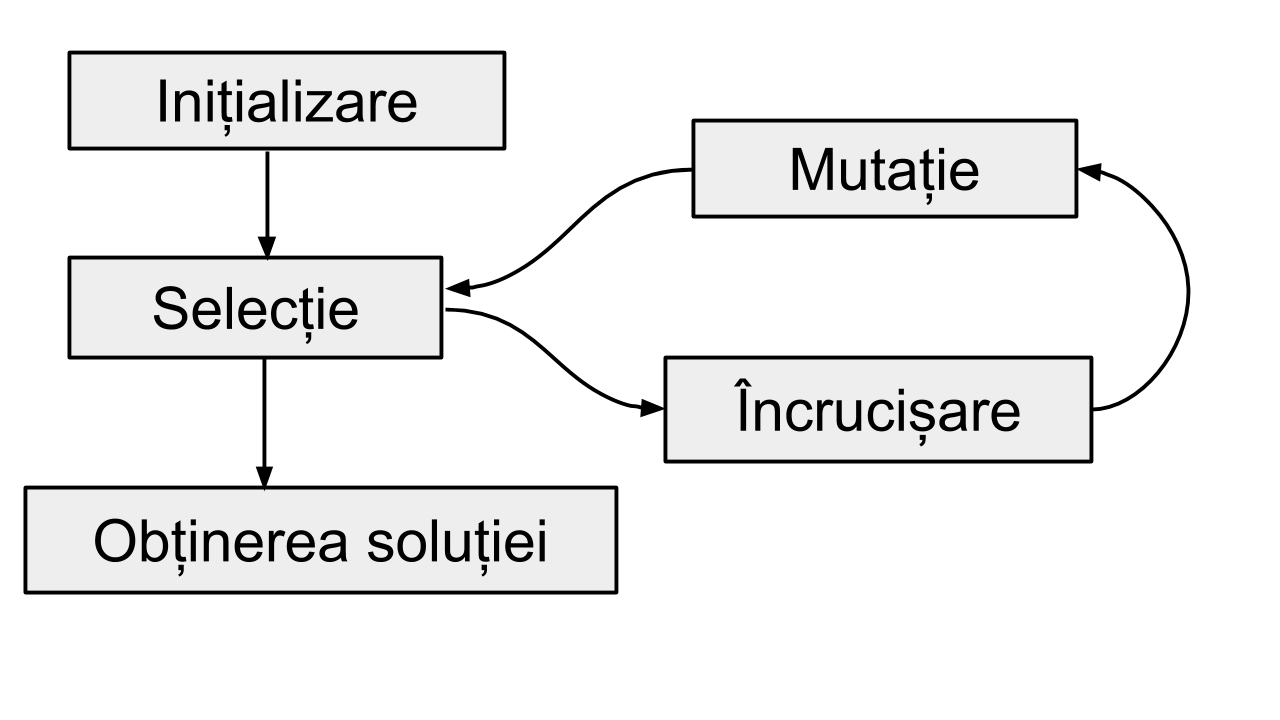
\includegraphics[
	width=10cm,
	height=6cm,
	keepaspectratio
]
{imagini/schema_algoritm_genetic.png}\\

\section{Pseudocod}

\begin{verbatim}
inițializează cu valori aleatorii populația inițială 
calculează valoarea funcției de optimizat pentru indivizii populației  
cât timp nu s-a îndeplinit condiția de oprire 
    aplică o metodă de selecție, pentru a crea populația 
    aplică operatorul genetic încrucișare, cu o anumită probabilitate 
    aplică operatorul genetic mutație, cu o anumită probabilitate 
    calculează valoarea funcției de optimizat pentru indivizii populației 
\end{verbatim}

Condiția de oprire poate fi atingerea unui număr de iterații stabilit inițial. De asemenea, se poate stabili ca algoritmul să se oprească atunci când nu se mai înregistrează îmbunătățiri în ceea ce privește calitatea soluțiilor furnizate.  
 
Soluția returnată de un algoritm genetic reprezintă cel mai bun individ întâlnit în evoluția populației.  

\clearpage